\documentclass[conference]{IEEEtran}

\usepackage{amsmath,amssymb,amsfonts,bm}
\usepackage{graphicx}
\usepackage{booktabs}
\usepackage{array}
\usepackage{multirow}
\usepackage{xcolor}
\usepackage{cite}
\usepackage{url}
\usepackage{mathtools}
\usepackage{stfloats}

\title{Trajectory Optimization and LQR-Based Terminal Stabilization for a Double Inverted Pendulum on a Cart}

\author{
\IEEEauthorblockN{Author Name}
\IEEEauthorblockA{Department of Mechanical and Aerospace Engineering\\
Advanced Robotics Course Project Report}
}

\begin{document}
\maketitle

\begin{abstract}
This paper presents a detailed version-2 write-up of the double inverted pendulum trajectory optimization project, extended from an open-loop swing-up planner to a hybrid controller that combines nonlinear trajectory optimization, trajectory-tracking linear quadratic regulation, and final equilibrium LQR stabilization. The manuscript is intentionally written as both a theory document and an implementation document. First, the cart--double-pendulum dynamics are derived in manipulator form and then converted into the six-state nonlinear model used in the code. Second, the finite-horizon swing-up problem is formulated from a calculus-of-variations and Pontryagin minimum principle perspective so that the roles of the Hamiltonian, costate dynamics, and stationarity condition are explicit. Third, the practical direct multiple-shooting transcription used in CasADi is described exactly, including the symbolic RK4 defects, warm-start reference, feedforward control guess, cost weights, solver settings, and path constraints. Fourth, the paper explains why the optimized open-loop plan by itself is not sufficient for reliable terminal balancing, and derives the local linear feedback laws used after planning. In particular, a continuous-time equilibrium LQR is obtained from local linearization and the algebraic Riccati equation, while a finite-horizon trajectory-tracking gain schedule is obtained from a backward Riccati recursion on time-varying linearizations along the optimized trajectory. The resulting controller can be interpreted as a practical TO\,+\,LQR architecture: nonlinear trajectory optimization performs the global swing-up task, the trajectory-tracking gains keep the execution close to the nominal plan, and a final equilibrium LQR maintains the unstable upright equilibrium after arrival. This report is written without page-limit compression and explains the notation, derivations, and implementation details at a level appropriate for an advanced robotics course in which optimal control derivations are expected to be shown explicitly.
\end{abstract}

\begin{IEEEkeywords}
trajectory optimization, calculus of variations, Pontryagin minimum principle, Hamiltonian, HJB, LQR, double inverted pendulum, cart-pole, CasADi
\end{IEEEkeywords}

\section{Introduction}
The double inverted pendulum on a cart is a representative underactuated robotic system in which a single horizontal cart force must coordinate translational motion of the base and rotational motion of two unstable pendulum links. Unlike a local balancing problem near an equilibrium, the swing-up task is fundamentally global and strongly nonlinear. Starting from a hanging configuration, the controller must inject energy, exploit inertial coupling, and steer the system into a neighborhood of the upright equilibrium from which a local stabilizer can take over.

This distinction between global motion generation and local stabilization is the central motivation for the present work. A local linear controller alone is inadequate from the downward configuration because the linear approximation only reflects the dynamics near a selected equilibrium. Conversely, a pure open-loop trajectory optimizer may produce an excellent finite-horizon plan in the model and still fail to hold the unstable upright state once the nominal horizon ends or once small modeling and execution deviations accumulate. The practical solution adopted in this project is therefore hybrid: use nonlinear trajectory optimization to generate the swing-up motion, then use LQR-based feedback to track the plan and stabilize the terminal equilibrium.

The existing project already contained a nonlinear CasADi trajectory optimizer for the double inverted pendulum. The purpose of this version-2 report is to document the extended formulation in a way that is suitable for an advanced robotics course. In particular, this manuscript does not stop at the code-level nonlinear program. It also includes the optimal-control derivation language that is often expected in a graduate course: variational reasoning, Hamiltonian construction, costate dynamics, stationarity conditions, and the relationship between Pontryagin's minimum principle and Hamilton--Jacobi theory.

The contributions of this manuscript are as follows.
\begin{enumerate}
\item The nonlinear dynamics are derived and explained using robotics notation consistent with the implementation.
\item The finite-horizon swing-up problem is formulated continuously, and the corresponding Hamiltonian and costate equations are written explicitly.
\item The direct multiple-shooting discretization used in the code is described exactly, including the reference warm start, feedforward input guess, path weights, terminal weights, and solver configuration.
\item The local terminal stabilizer is derived from linearization and the continuous-time algebraic Riccati equation.
\item The trajectory-tracking feedback implemented in the current code is interpreted as a finite-horizon LQR-style backward Riccati recursion computed along the optimized state and control trajectory.
\item The paper clarifies what changed from the original trajectory-optimization-only implementation: the nonlinear trajectory optimizer itself was preserved, while the execution layer was extended with trajectory-tracking and final-equilibrium stabilization.
\end{enumerate}

The rest of the paper proceeds from modeling, to continuous optimal control theory, to numerical transcription, and finally to hybrid control synthesis and implementation details.

\IfFileExists{../figures/trajopt_lqr_response.pdf}{
\begin{figure*}[!t]
\centering
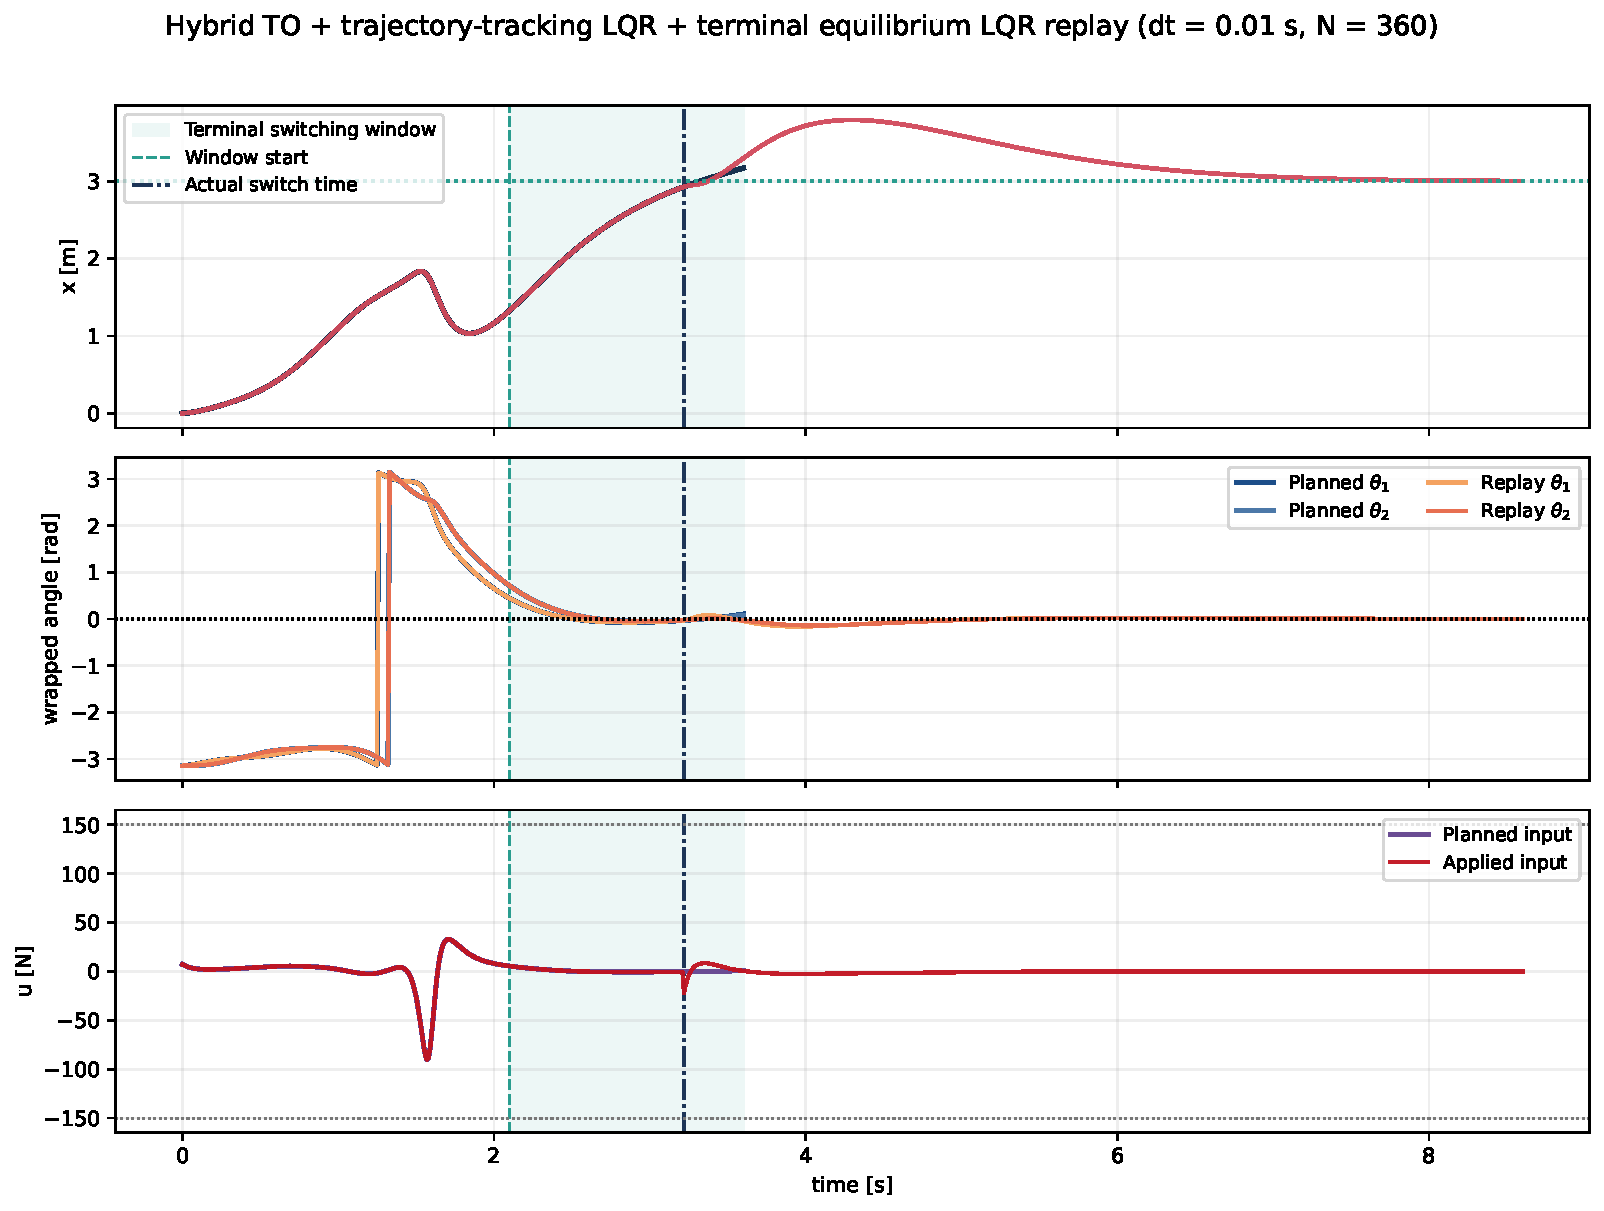
\includegraphics[width=0.96\textwidth]{../figures/trajopt_lqr_response.pdf}
\caption{Hybrid replay for the current controller architecture using the final figure-generation settings $N=360$, $\Delta t=0.01$~s, and $T_{\mathrm{hold}}=5.0$~s. The shaded region denotes the \emph{terminal switching window}, not the exact interval in which the controller has already switched. The dashed vertical line marks the start of the window at $t=2.1$~s, while the dash-dotted vertical line marks the actual switching instant at approximately $t=3.22$~s. Thus the optimizer still plans through $t=3.6$~s, but the controller is allowed to hand over earlier if the state has already entered the local basin of attraction of the final equilibrium LQR.}
\label{fig:hybrid_response}
\end{figure*}
}{}

\section{System Model and Notation}
\subsection{Coordinates and State}
Let the generalized coordinate vector be
\begin{equation}
\bm{q} =
\begin{bmatrix}
x & \theta_1 & \theta_2
\end{bmatrix}^{\top},
\end{equation}
where $x$ is the horizontal cart position, $\theta_1$ is the angle of the first pendulum link, and $\theta_2$ is the angle of the second pendulum link. In the repository convention, both angles are measured from the upright direction. Hence
\begin{equation}
\theta_1 = \theta_2 = 0
\end{equation}
is the upright equilibrium, while the nominal hanging pose is near
\begin{equation}
\theta_1 = \theta_2 = \pi.
\end{equation}

The full state vector is
\begin{equation}
\bm{x} =
\begin{bmatrix}
x & \theta_1 & \theta_2 & \dot{x} & \dot{\theta}_1 & \dot{\theta}_2
\end{bmatrix}^{\top}
\in \mathbb{R}^{6},
\end{equation}
and the scalar control input is the horizontal cart force
\begin{equation}
u \in \mathbb{R}.
\end{equation}

The default physical parameter structure in the model is
\begin{align}
m_0 &= 1.0 \text{ kg}, &
m_1 &= 0.2 \text{ kg}, &
m_2 &= 0.2 \text{ kg}, \\
l_1 &= 0.5 \text{ m}, &
l_2 &= 0.5 \text{ m}, &
g &= 9.81 \text{ m/s}^2.
\end{align}
In the current TO\,+\,LQR demo script, these are combined with the modified damping and saturation values
\begin{align}
d_x &= 1.0, &
d_1 &= 0.1, &
d_2 &= 0.01, &
u_{\max} &= 150 \text{ N}.
\end{align}

\subsection{Kinematics}
The cart position in the plane is
\begin{equation}
\bm{p}_c =
\begin{bmatrix}
x \\ 0
\end{bmatrix}.
\end{equation}
The first link tip position is
\begin{equation}
\bm{p}_1 = \bm{p}_c +
\begin{bmatrix}
l_1 \sin \theta_1 \\
l_1 \cos \theta_1
\end{bmatrix},
\end{equation}
and the second link tip position is
\begin{equation}
\bm{p}_2 = \bm{p}_1 +
\begin{bmatrix}
l_2 \sin \theta_2 \\
l_2 \cos \theta_2
\end{bmatrix}.
\end{equation}

This global-angle convention is simple and matches the implementation. It also implies that angular errors should not be treated as ordinary Euclidean differences. Instead, angle errors must be wrapped into the principal interval $(-\pi,\pi]$, which is why the code uses the function
\begin{equation}
\mathrm{wrap}(\theta) = (\theta + \pi)\bmod 2\pi - \pi.
\end{equation}

\subsection{Manipulator-Form Dynamics}
The implemented equations of motion are written in second-order manipulator form,
\begin{equation}
\bm{M}(\bm{q}) \ddot{\bm{q}} = \bm{\tau}(\bm{q}, \dot{\bm{q}}, u),
\label{eq:manipulator_form}
\end{equation}
where the mass matrix is
\begin{equation}
\resizebox{\columnwidth}{!}{$
\bm{M}(\bm{q}) =
\begin{bmatrix}
m_0 + m_1 + m_2 & (m_1+m_2)l_1\cos\theta_1 & m_2 l_2 \cos\theta_2 \\
(m_1+m_2)l_1\cos\theta_1 & (m_1+m_2)l_1^2 & m_2 l_1 l_2 \cos(\theta_1-\theta_2) \\
m_2 l_2 \cos\theta_2 & m_2 l_1 l_2 \cos(\theta_1-\theta_2) & m_2 l_2^2
\end{bmatrix}
$}
\end{equation}
and the generalized-force vector is
\begin{equation}
\resizebox{\columnwidth}{!}{$
\bm{\tau} =
\begin{bmatrix}
u - d_x \dot{x} + (m_1+m_2)l_1 \sin\theta_1 \dot{\theta}_1^2 + m_2 l_2 \sin\theta_2 \dot{\theta}_2^2 \\
- d_1 \dot{\theta}_1 - m_2 l_1 l_2 \sin(\theta_1-\theta_2)\dot{\theta}_2^2 + (m_1+m_2) g l_1 \sin\theta_1 \\
- d_2 \dot{\theta}_2 + m_2 l_1 l_2 \sin(\theta_1-\theta_2)\dot{\theta}_1^2 + m_2 g l_2 \sin\theta_2
\end{bmatrix}
$}.
\label{eq:generalized_forces}
\end{equation}

The physical interpretation is standard but important. The diagonal of $\bm{M}(\bm{q})$ represents inertia associated with each generalized coordinate. The off-diagonal terms encode dynamic coupling. Since the single actuator acts only through $u$ in the cart coordinate, all pendulum motion must be induced indirectly through these coupling terms.

Solving \eqref{eq:manipulator_form} for $\ddot{\bm{q}}$ gives the first-order nonlinear state dynamics
\begin{equation}
\dot{\bm{x}} = \bm{f}(\bm{x},u)
=
\begin{bmatrix}
\dot{x} &
\dot{\theta}_1 &
\dot{\theta}_2 &
\ddot{x} &
\ddot{\theta}_1 &
\ddot{\theta}_2
\end{bmatrix}^{\top}.
\end{equation}
The implementation clips the force before inserting it into the dynamics:
\begin{equation}
u_{\mathrm{sat}} = \mathrm{clip}(u,-u_{\max},u_{\max}).
\end{equation}

\section{Continuous Optimal Control Formulation}
\subsection{Swing-Up as a Finite-Horizon Problem}
The continuous-time swing-up problem may be written as follows. Given an initial state $\bm{x}(0)=\bm{x}_0$, find a control signal $u(\cdot)$ over $t\in[0,T]$ that minimizes
\begin{equation}
J[u] = \phi(\bm{x}(T)) + \int_{0}^{T} L(\bm{x}(t),u(t),t)\,dt
\label{eq:continuous_cost}
\end{equation}
subject to the nonlinear dynamics
\begin{equation}
\dot{\bm{x}}(t) = \bm{f}(\bm{x}(t),u(t)).
\label{eq:continuous_dynamics}
\end{equation}

Here $L$ is the running cost and $\phi$ is the terminal cost. In words, the controller is trying to make the entire trajectory economical according to $L$, while also arriving in a desirable terminal state according to $\phi$.

In the current project, the goal state is
\begin{equation}
\bm{x}^{\star} =
\begin{bmatrix}
3 & 0 & 0 & 0 & 0 & 0
\end{bmatrix}^{\top},
\end{equation}
meaning the cart should arrive at $x=3$ m and both links should be upright with near-zero velocity.

\subsection{Calculus-of-Variations Viewpoint}
To expose the optimality conditions expected in an advanced robotics course, introduce the augmented functional
\begin{equation}
\bar{J}
=
\phi(\bm{x}(T))
+
\int_0^T
\left[
L(\bm{x},u,t)
+
\bm{\lambda}^{\top}(t)\big(\bm{f}(\bm{x},u)-\dot{\bm{x}}\big)
\right] dt,
\label{eq:augmented_functional}
\end{equation}
where $\bm{\lambda}(t)\in\mathbb{R}^6$ is the costate. The role of the costate is to enforce the state dynamics as a variational constraint.

Define the Hamiltonian
\begin{equation}
H(\bm{x},u,\bm{\lambda},t)
=
L(\bm{x},u,t)+\bm{\lambda}^{\top}\bm{f}(\bm{x},u).
\label{eq:hamiltonian}
\end{equation}
Then \eqref{eq:augmented_functional} becomes
\begin{equation}
\bar{J}
=
\phi(\bm{x}(T))
+
\int_0^T
\left[
H(\bm{x},u,\bm{\lambda},t)
-\bm{\lambda}^{\top}\dot{\bm{x}}
\right] dt.
\end{equation}

Now take the first variation. Varying the state, input, and costate gives
\begin{align}
\delta \bar{J}
&=
\nabla \phi(\bm{x}(T))^{\top}\delta \bm{x}(T)
+
\int_0^T
\left[
\frac{\partial H}{\partial \bm{x}}^{\top}\delta \bm{x}
+
\frac{\partial H}{\partial u}\delta u
+
\frac{\partial H}{\partial \bm{\lambda}}^{\top}\delta \bm{\lambda}
- \delta\bm{\lambda}^{\top}\dot{\bm{x}}
- \bm{\lambda}^{\top}\delta\dot{\bm{x}}
\right] dt.
\end{align}
Integrating the last term by parts,
\begin{equation}
\int_0^T -\bm{\lambda}^{\top}\delta \dot{\bm{x}}\,dt
=
\left[-\bm{\lambda}^{\top}\delta \bm{x}\right]_{0}^{T}
+
\int_0^T \dot{\bm{\lambda}}^{\top}\delta \bm{x}\,dt.
\end{equation}
Since the initial state is fixed, $\delta \bm{x}(0)=0$. Therefore
\begin{align}
\delta \bar{J}
&=
\big(\nabla \phi(\bm{x}(T))-\bm{\lambda}(T)\big)^{\top}\delta \bm{x}(T)
\nonumber\\
&\quad
+
\int_0^T
\left[
\left(\frac{\partial H}{\partial \bm{x}}+\dot{\bm{\lambda}}\right)^{\top}\delta \bm{x}
+
\frac{\partial H}{\partial u}\delta u
+
\left(\frac{\partial H}{\partial \bm{\lambda}}-\dot{\bm{x}}\right)^{\top}\delta \bm{\lambda}
\right] dt.
\label{eq:first_variation}
\end{align}
Because the variations are arbitrary, the stationarity of \eqref{eq:first_variation} yields the familiar necessary conditions:
\begin{align}
\dot{\bm{x}} &= \frac{\partial H}{\partial \bm{\lambda}} = \bm{f}(\bm{x},u),
\label{eq:state_eq_pmp}
\\
\dot{\bm{\lambda}} &= -\frac{\partial H}{\partial \bm{x}},
\label{eq:costate_eq_pmp}
\\
0 &= \frac{\partial H}{\partial u},
\label{eq:stationarity_pmp}
\\
\bm{\lambda}(T) &= \nabla \phi(\bm{x}(T)).
\label{eq:terminal_costate}
\end{align}

Equation \eqref{eq:costate_eq_pmp} is the costate equation that the professor would expect to see in a variational derivation. Equation \eqref{eq:stationarity_pmp} is the pointwise optimality condition. Together, \eqref{eq:state_eq_pmp}--\eqref{eq:terminal_costate} define a two-point boundary-value problem: the state is known at the initial time, the costate is known at the terminal time, and the two must be solved jointly.

\subsection{Pontryagin Minimum Principle Interpretation}
The variational calculation above is the standard entry point to Pontryagin's minimum principle (PMP). PMP states that if $u^{\star}(t)$ is an optimal control and $\bm{x}^{\star}(t)$ is its corresponding state trajectory, then there exists a costate $\bm{\lambda}^{\star}(t)$ such that
\begin{align}
\dot{\bm{x}}^{\star}(t) &= \frac{\partial H}{\partial \bm{\lambda}}
\Big|_{(\bm{x}^{\star},u^{\star},\bm{\lambda}^{\star})},
\\
\dot{\bm{\lambda}}^{\star}(t) &= -\frac{\partial H}{\partial \bm{x}}
\Big|_{(\bm{x}^{\star},u^{\star},\bm{\lambda}^{\star})},
\\
u^{\star}(t) &\in \arg\min_{u\in\mathcal{U}}
H(\bm{x}^{\star}(t),u,\bm{\lambda}^{\star}(t),t),
\end{align}
with the terminal condition
\begin{equation}
\bm{\lambda}^{\star}(T)=\nabla \phi(\bm{x}^{\star}(T)).
\end{equation}

For this project, the admissible control set is the saturation interval
\begin{equation}
\mathcal{U} = [-u_{\max},u_{\max}].
\end{equation}
Hence the minimizing input must also respect hard actuator bounds.

The importance of PMP in this report is not that the code directly solves the costate boundary-value problem. It does not. Instead, the significance is conceptual: the CasADi nonlinear program is a numerical transcription of precisely this constrained finite-horizon optimal control problem. The multiple-shooting variables, defect constraints, and finite-dimensional objective are the discrete counterparts of the continuous equations above.

\subsection{Hamilton--Jacobi--Bellman Viewpoint}
An equally important theoretical perspective is dynamic programming. Let
\begin{equation}
V(\bm{x},t)=
\min_{u(\cdot)}
\left[
\phi(\bm{x}(T))
+
\int_t^T L(\bm{x}(\tau),u(\tau),\tau)\,d\tau
\right]
\end{equation}
be the value function. Then $V$ satisfies the Hamilton--Jacobi--Bellman (HJB) equation
\begin{equation}
-\frac{\partial V}{\partial t}(\bm{x},t)
=
\min_{u\in\mathcal{U}}
\left[
L(\bm{x},u,t)
+
\nabla_{\bm{x}}V(\bm{x},t)^{\top}\bm{f}(\bm{x},u)
\right],
\label{eq:hjb}
\end{equation}
with terminal boundary condition
\begin{equation}
V(\bm{x},T)=\phi(\bm{x}).
\end{equation}

Equation \eqref{eq:hjb} is the dynamic-programming counterpart to PMP. The term inside the minimum is exactly the Hamiltonian with the identification
\begin{equation}
\bm{\lambda}(t)=\nabla_{\bm{x}}V(\bm{x}(t),t).
\end{equation}
Thus PMP and HJB are not competing theories; they are complementary ways of expressing the same optimal-control structure.

The reason HJB is particularly relevant here is that LQR can be derived directly from it. Once the dynamics are linearized near an equilibrium and the cost is approximated quadratically, the value function becomes quadratic, and the HJB PDE reduces to a Riccati equation. That is precisely the bridge from nonlinear optimal control to the local LQR stabilizer used at the end of the trajectory.

\section{Practical Nonlinear Trajectory Optimization Used in the Code}
\subsection{Reference Warm Start}
The code warm-starts the nonlinear program using a smooth cubic interpolation between initial and goal states. Define the normalized horizon coordinate
\begin{equation}
\tau_k = \frac{k}{N}, \qquad k=0,\ldots,N,
\end{equation}
and the smoothstep profile
\begin{equation}
s(\tau)=3\tau^2-2\tau^3.
\end{equation}
Then the reference state is
\begin{align}
x_k^{\mathrm{ref}} &= x_0 + (x^{\star}-x_0)s(\tau_k), \\
\theta_{1,k}^{\mathrm{ref}} &= \theta_{1,0}+(\theta_1^{\star}-\theta_{1,0})s(\tau_k), \\
\theta_{2,k}^{\mathrm{ref}} &= \theta_{2,0}+(\theta_2^{\star}-\theta_{2,0})s(\tau_k),
\end{align}
while the reference velocities are set to zero.

This reference is not dynamically feasible. It is simply a good initial guess that keeps the optimizer away from pathological initializations.

\IfFileExists{../figures/trajopt_reference.pdf}{
\begin{figure}[!t]
\centering
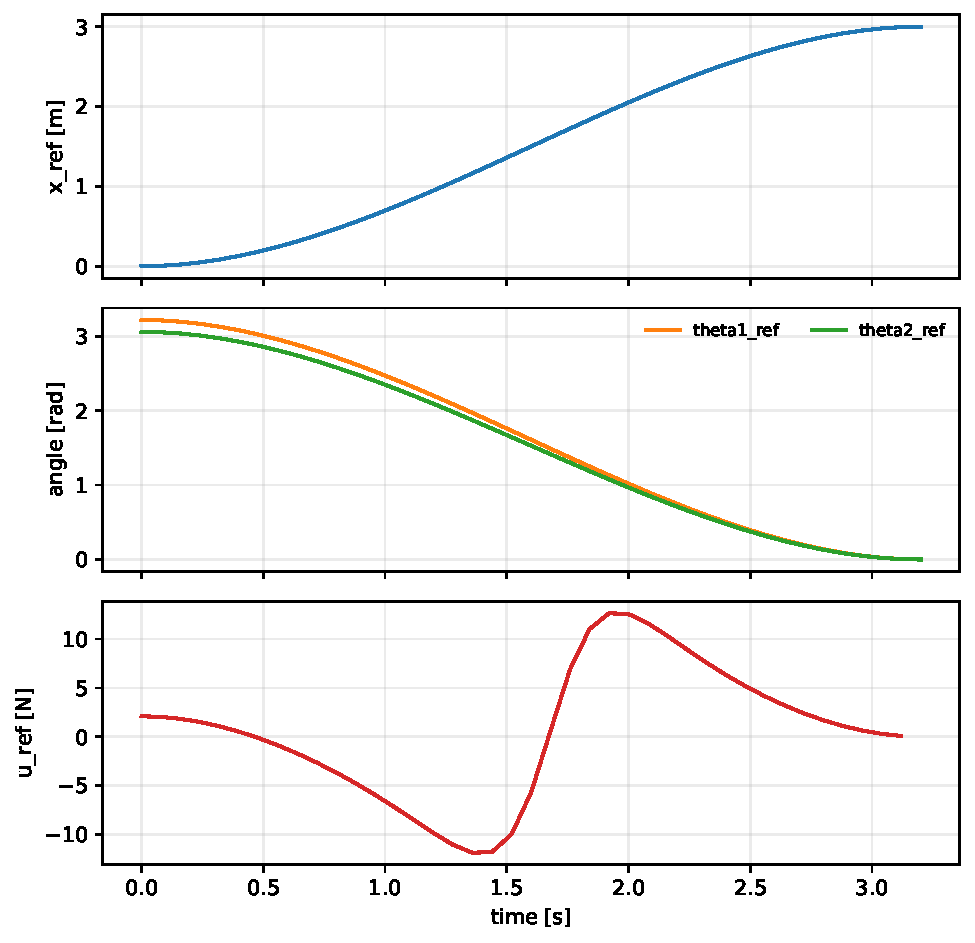
\includegraphics[width=\columnwidth]{../figures/trajopt_reference.pdf}
\caption{Smooth swing-up reference and feedforward input initialization used to warm-start the CasADi trajectory optimizer. Even though this reference is not dynamically feasible, it gives the nonlinear program a physically meaningful starting point.}
\label{fig:trajopt_reference_v2}
\end{figure}
}{}

\subsection{Feedforward Input Initialization}
For each reference state, a scalar feedforward input is computed by the bounded one-dimensional optimization
\begin{equation}
u_k^{\mathrm{ref}}
\in
\arg\min_{u\in[-u_{\max},u_{\max}]}
\left\|
\ddot{\bm{q}}(\bm{x}_k^{\mathrm{ref}},u)
\right\|_2^2.
\label{eq:feedforward_guess}
\end{equation}
Intuitively, this chooses an input that makes the reference configuration as dynamically quiet as possible.

\subsection{Decision Variables}
The direct multiple-shooting transcription introduces the state matrix
\begin{equation}
\bm{X}=
\begin{bmatrix}
\bm{x}_0 & \bm{x}_1 & \cdots & \bm{x}_N
\end{bmatrix}
\in \mathbb{R}^{6\times(N+1)}
\end{equation}
and the control matrix
\begin{equation}
\bm{U}=
\begin{bmatrix}
u_0 & u_1 & \cdots & u_{N-1}
\end{bmatrix}
\in \mathbb{R}^{1\times N}.
\end{equation}
The initial node is constrained by
\begin{equation}
\bm{x}_0 = \bm{x}_{\mathrm{init}}.
\end{equation}

\subsection{RK4 Defect Constraints}
Dynamic feasibility is enforced with a symbolic RK4 step. For each $k=0,\ldots,N-1$,
\begin{equation}
\bm{x}_{k+1} = \Phi_{\mathrm{RK4}}(\bm{x}_k,u_k),
\label{eq:defect_constraint}
\end{equation}
where
\begin{align}
\bm{k}_1 &= \bm{f}(\bm{x}_k,u_k), \\
\bm{k}_2 &= \bm{f}\!\left(\bm{x}_k+\frac{\Delta t}{2}\bm{k}_1,u_k\right), \\
\bm{k}_3 &= \bm{f}\!\left(\bm{x}_k+\frac{\Delta t}{2}\bm{k}_2,u_k\right), \\
\bm{k}_4 &= \bm{f}\!\left(\bm{x}_k+\Delta t\bm{k}_3,u_k\right), \\
\Phi_{\mathrm{RK4}}(\bm{x}_k,u_k) &=
\bm{x}_k + \frac{\Delta t}{6}\left(\bm{k}_1+2\bm{k}_2+2\bm{k}_3+\bm{k}_4\right).
\end{align}

\subsection{Stage and Terminal Cost Used in the Implementation}
The repository uses the following quadratic and periodic cost components:
\begin{align}
\bm{Q}_{\mathrm{path}} &= \mathrm{diag}(8.0,\,0,\,0,\,0.35,\,0.2,\,0.2), \\
\bm{Q}_{\mathrm{term}} &= \mathrm{diag}(65.0,\,0,\,0,\,5.0,\,3.0,\,3.0),
\end{align}
with angular penalties
\begin{align}
w_{\theta,\mathrm{path}} &= 10.0, \\
w_{\theta,\mathrm{term}} &= 140.0,
\end{align}
and input regularization
\begin{align}
w_u &= 0.003, \\
w_{\Delta u} &= 0.0008.
\end{align}

The angular mismatch is measured with the periodic function
\begin{equation}
\ell_{\mathrm{ang}}(\theta,\theta_{\mathrm{ref}})
=
1-\cos(\theta-\theta_{\mathrm{ref}}),
\end{equation}
which avoids discontinuities from angle wrapping.

Thus the implemented finite-dimensional objective is
\begin{align}
J_{\mathrm{NLP}}
&=
\sum_{k=0}^{N-1}
\Big[
(\bm{x}_k-\bm{x}^{\mathrm{ref}}_k)^{\top}\bm{Q}_{\mathrm{path}}(\bm{x}_k-\bm{x}^{\mathrm{ref}}_k)
\nonumber\\
&\qquad
+ w_{\theta,\mathrm{path}}\ell_{\mathrm{ang}}(\theta_{1,k},\theta^{\mathrm{ref}}_{1,k})
+ w_{\theta,\mathrm{path}}\ell_{\mathrm{ang}}(\theta_{2,k},\theta^{\mathrm{ref}}_{2,k})
\nonumber\\
&\qquad
+ w_u (u_k-u_k^{\mathrm{ref}})^2
+ w_{\Delta u}(u_k-u_{k-1})^2
\Big]
\nonumber\\
&\quad
+ (\bm{x}_N-\bm{x}^{\star})^{\top}\bm{Q}_{\mathrm{term}}(\bm{x}_N-\bm{x}^{\star})
\nonumber\\
&\quad
+ w_{\theta,\mathrm{term}}\ell_{\mathrm{ang}}(\theta_{1,N},\theta_1^{\star})
+ w_{\theta,\mathrm{term}}\ell_{\mathrm{ang}}(\theta_{2,N},\theta_2^{\star}),
\label{eq:implemented_nlp_cost}
\end{align}
where the smoothing term is omitted at $k=0$.

\subsection{Constraints and Solver Configuration}
The control bounds are
\begin{equation}
-u_{\max}\le u_k \le u_{\max}.
\end{equation}
If enabled, cart position bounds are imposed as
\begin{equation}
x_{\min}\le x_k \le x_{\max}.
\end{equation}
In the current demo script, the replay stage uses
\begin{equation}
(x_{\min},x_{\max}) = (-2.5,7.5),
\end{equation}
while the TO solve may or may not enforce those bounds depending on the command-line option.

The CasADi frontend uses IPOPT when available, with
\begin{align}
\texttt{max\_iter} &= 2000, \\
\texttt{tol} &= 10^{-4}, \\
\texttt{acceptable\_tol} &= 10^{-3}, \\
\texttt{acceptable\_iter} &= 8.
\end{align}
The final visualization and hybrid replay results in this report use
\begin{equation}
N=360, \qquad \Delta t=0.01 \text{ s},
\end{equation}
which yields a planning horizon of
\begin{equation}
T = N \Delta t = 3.6 \text{ s}.
\end{equation}
Thus the horizon duration is unchanged from the earlier $N=120$, $\Delta t=0.03$ configuration, but the trajectory is sampled three times more densely in time, which produces visibly smoother plots and a finer direct multiple-shooting discretization.

\begin{table}[!t]
\caption{Final Parameters Used for the Version-2 TO\,+\,LQR Figures}
\label{tab:finalparams}
\centering
\begin{tabular}{l l}
\toprule
Item & Value \\
\midrule
TO horizon steps $N$ & 360 \\
TO timestep $\Delta t$ & 0.01 s \\
Planning horizon $T$ & 3.6 s \\
Post-plan hold time $T_{\mathrm{hold}}$ & 5.0 s \\
Track bounds & $[-2.5,\,7.5]$ m \\
Cart damping $d_x$ & 1.0 \\
Joint damping $(d_1,d_2)$ & $(0.1,\,0.01)$ \\
Force limit $u_{\max}$ & 150 N \\
$\bm{Q}_{\mathrm{path}}$ & $\mathrm{diag}(8,0,0,0.35,0.2,0.2)$ \\
$\bm{Q}_{\mathrm{term}}$ & $\mathrm{diag}(65,0,0,5,3,3)$ \\
$w_{\theta,\mathrm{path}}$ & 10.0 \\
$w_{\theta,\mathrm{term}}$ & 140.0 \\
$w_u$ & 0.003 \\
$w_{\Delta u}$ & 0.0008 \\
Tracking $\bm{Q}_{\mathrm{track}}$ & $\mathrm{diag}(20,140,140,8,18,18)$ \\
Tracking $\bm{R}_{\mathrm{track}}$ & 0.8 \\
Equilibrium LQR $\bm{Q}$ & $\mathrm{diag}(30,220,220,18,32,32)$ \\
Equilibrium LQR $\bm{R}$ & 0.6 \\
Switch thresholds & $(0.16 \text{ rad},\,0.8,\,0.25 \text{ m})$ \\
Terminal switch window & 1.5 s \\
\bottomrule
\end{tabular}
\end{table}

\IfFileExists{../figures/trajopt_plan.pdf}{
\begin{figure}[!t]
\centering

\includegraphics[width=\columnwidth]{../figures/trajopt_plan.pdf}
\caption{Optimized swing-up plan produced by the nonlinear trajectory optimization module. This is the nominal motion that the version-2 controller tracks before switching to terminal stabilization.}
\label{fig:trajopt_plan_v2}
\end{figure}
}{}

\section{Why Open-Loop Trajectory Optimization Alone Is Not Enough}
Although the NLP in \eqref{eq:implemented_nlp_cost} can produce a feasible swing-up plan, the plan is still fundamentally finite horizon and model based. Two practical limitations follow immediately.

First, the optimizer solves a \emph{terminal-reaching} problem, not an infinite-horizon stabilization problem. Even if the terminal state is near upright, the optimization itself does not guarantee that the system will remain there after the horizon ends.

Second, the optimized state sequence and input sequence are only nominal. During execution, even small mismatch in damping, numerical integration, or phase timing can move the nonlinear system away from the nominal path. For an unstable terminal equilibrium, these deviations can grow rapidly.

This is exactly why a TO\,+\,LQR architecture is natural. The trajectory optimizer supplies a globally meaningful nominal motion, and the LQR laws supply local feedback authority. In other words,
\begin{equation}
\text{TO plans how to arrive, \qquad LQR ensures how to stay.}
\end{equation}

\section{Local Linearization and Final Equilibrium LQR}
\subsection{Linearization}
Let $(\bm{x}_{\mathrm{eq}},u_{\mathrm{eq}})$ denote the upright equilibrium pair. In the current task,
\begin{equation}
\bm{x}_{\mathrm{eq}} =
\begin{bmatrix}
3 & 0 & 0 & 0 & 0 & 0
\end{bmatrix}^{\top},
\qquad
u_{\mathrm{eq}} = 0.
\end{equation}
Linearizing the nonlinear system around this operating point yields
\begin{equation}
\delta \dot{\bm{x}} = \bm{A}\,\delta\bm{x} + \bm{B}\,\delta u,
\label{eq:linearized_eq}
\end{equation}
where
\begin{align}
\bm{A} &= \left.\frac{\partial \bm{f}}{\partial \bm{x}}\right|_{(\bm{x}_{\mathrm{eq}},u_{\mathrm{eq}})}, \\
\bm{B} &= \left.\frac{\partial \bm{f}}{\partial u}\right|_{(\bm{x}_{\mathrm{eq}},u_{\mathrm{eq}})}.
\end{align}
The implementation computes these Jacobians numerically with centered finite differences.

\subsection{LQR Cost and HJB Derivation}
For the linearized system \eqref{eq:linearized_eq}, define the infinite-horizon quadratic cost
\begin{equation}
J_{\mathrm{LQR}}
=
\int_0^{\infty}
\left(
\delta\bm{x}^{\top}\bm{Q}\delta\bm{x}
+
\delta u^{\top}\bm{R}\delta u
\right)dt,
\end{equation}
with
\begin{align}
\bm{Q} &= \mathrm{diag}(30,\,220,\,220,\,18,\,32,\,32), \\
\bm{R} &= [0.6].
\end{align}

Now derive the feedback law by the HJB method. Assume the value function is quadratic:
\begin{equation}
V(\delta\bm{x}) = \delta\bm{x}^{\top}\bm{S}\delta\bm{x},
\end{equation}
where $\bm{S}=\bm{S}^{\top}\succcurlyeq 0$. Then
\begin{equation}
\nabla V(\delta\bm{x}) = 2\bm{S}\delta\bm{x}.
\end{equation}
Substituting into the stationary HJB equation gives
\begin{align}
0 &=
\min_{\delta u}
\Big[
\delta\bm{x}^{\top}\bm{Q}\delta\bm{x}
+
\delta u^{\top}\bm{R}\delta u
+
2\delta\bm{x}^{\top}\bm{S}(\bm{A}\delta\bm{x}+\bm{B}\delta u)
\Big].
\end{align}
Differentiate with respect to $\delta u$:
\begin{equation}
2\bm{R}\delta u + 2\bm{B}^{\top}\bm{S}\delta\bm{x}=0.
\end{equation}
Therefore
\begin{equation}
\delta u = -\bm{K}\delta\bm{x},
\qquad
\bm{K}=\bm{R}^{-1}\bm{B}^{\top}\bm{S}.
\label{eq:lqr_gain}
\end{equation}
Substituting back into HJB yields the continuous-time algebraic Riccati equation (CARE):
\begin{equation}
\bm{A}^{\top}\bm{S}
+
\bm{S}\bm{A}
- \bm{S}\bm{B}\bm{R}^{-1}\bm{B}^{\top}\bm{S}
+
\bm{Q}
= 0.
\label{eq:care}
\end{equation}

This is exactly the LQR relation one would want to connect to Hamilton--Jacobi theory in a course report. The code solves \eqref{eq:care} with \texttt{scipy.linalg.solve\_continuous\_are} and then computes the gain from \eqref{eq:lqr_gain}. The implemented equilibrium control law is
\begin{equation}
u = u_{\mathrm{eq}} - \bm{K}\,\delta\bm{x}.
\end{equation}

\subsection{Direct Link Between the HJB Derivation and the Implemented LQR}
Because the theoretical derivation can otherwise feel detached from the code, it is worth making the connection explicit. The final equilibrium LQR used in the implementation is precisely the controller obtained by applying the HJB derivation above to the linearized upright dynamics. In other words,
\begin{align}
\text{nonlinear system } \bm{f}(\bm{x},u)
&\xrightarrow{\text{linearize at }(\bm{x}_{\mathrm{eq}},u_{\mathrm{eq}})}
(\bm{A},\bm{B}),
\\
(\bm{A},\bm{B}),(\bm{Q},\bm{R})
&\xrightarrow{\text{HJB with }V=\delta\bm{x}^{\top}\bm{S}\delta\bm{x}}
\bm{S},
\\
\bm{S}
&\xrightarrow{\bm{K}=\bm{R}^{-1}\bm{B}^{\top}\bm{S}}
\bm{K}_{\mathrm{eq}}.
\end{align}
Therefore the matrix \texttt{s} stored in the code's \texttt{LQRGain} structure is the numerical Riccati solution $\bm{S}$, and the matrix \texttt{k} is exactly the gain $\bm{K}_{\mathrm{eq}}$ predicted by the HJB derivation. The code is not merely ``inspired by'' HJB at this stage; it is implementing the Riccati solution that HJB produces for the local quadratic approximation.

\section{Trajectory-Tracking LQR Along the Optimized Swing-Up}
\subsection{Why a Single Final LQR Is Not Sufficient During the Entire Swing-Up}
The final equilibrium LQR is valid only near the upright equilibrium. It is not appropriate for the entire swing-up because the system spends most of the maneuver far from the local linearization point. What is needed during the transient is a trajectory-tracking controller around the optimized nominal state and control sequence
\begin{equation}
\{\bm{x}_0^{\star},\bm{x}_1^{\star},\ldots,\bm{x}_N^{\star}\},
\qquad
\{u_0^{\star},u_1^{\star},\ldots,u_N^{\star}\}.
\end{equation}

\subsection{Time-Varying Linearization Along the Plan}
At each discrete stage $k$, linearize around the nominal pair $(\bm{x}_k^{\star},u_k^{\star})$:
\begin{equation}
\delta \dot{\bm{x}} = \bm{A}_k \delta\bm{x} + \bm{B}_k \delta u.
\end{equation}
The implementation uses the finite-difference Jacobian routine already available in the repository, evaluated at each planned state and input.

With timestep $\Delta t_k = t_{k+1}-t_k$, the code forms a first-order discrete approximation
\begin{align}
\bm{A}_{d,k} &= \bm{I} + \Delta t_k \bm{A}_k, \\
\bm{B}_{d,k} &= \Delta t_k \bm{B}_k.
\end{align}

\subsection{Backward Riccati Recursion}
The trajectory-tracking controller implemented in the current code uses the quadratic weights
\begin{align}
\bm{Q}_{\mathrm{track}} &= \mathrm{diag}(20,\,140,\,140,\,8,\,18,\,18), \\
\bm{R}_{\mathrm{track}} &= [0.8].
\end{align}
Starting from the final Riccati matrix
\begin{equation}
\bm{S}_N = \bm{S}_{\mathrm{eq}},
\end{equation}
where $\bm{S}_{\mathrm{eq}}$ is the CARE solution of the final equilibrium LQR, the code runs the backward recursion
\begin{align}
\bm{G}_k &=
\bm{R}_{\mathrm{track}} + \bm{B}_{d,k}^{\top}\bm{S}_{k+1}\bm{B}_{d,k},
\\
\bm{K}_k &=
\bm{G}_k^{-1}\bm{B}_{d,k}^{\top}\bm{S}_{k+1}\bm{A}_{d,k},
\label{eq:tvlqr_gain}
\\
\bm{S}_k &=
\bm{Q}_{\mathrm{track}}
+
\bm{A}_{d,k}^{\top}\bm{S}_{k+1}(\bm{A}_{d,k}-\bm{B}_{d,k}\bm{K}_k).
\label{eq:tvlqr_riccati}
\end{align}

This is the discrete finite-horizon LQR recursion. Conceptually, it is a local approximation to solving HJB backward in time along the nominal trajectory. Thus even though the implementation is practical and numerical, it still has a clean theoretical interpretation within the dynamic-programming framework.

For the final figures generated with $N=360$ and $\Delta t=0.01$~s, this recursion is carried out over 361 nominal states and 361 stored control samples, which yields a comparatively smooth scheduled gain sequence for trajectory tracking.

\subsection{Implemented Tracking Control Law}
Let the reference state at execution time $t$ be obtained from linear interpolation of the planned states, and let $k(t)$ denote the associated index. The tracking error is
\begin{equation}
\delta\bm{x}_{\mathrm{track}}(t)
=
\bm{x}(t)-\bm{x}^{\star}(t),
\end{equation}
with the angular components wrapped into $(-\pi,\pi]$. The controller then applies
\begin{equation}
u(t)=u_{k(t)}^{\star} - \bm{K}_{k(t)}\,\delta\bm{x}_{\mathrm{track}}(t).
\label{eq:tracking_control_law}
\end{equation}

Equation \eqref{eq:tracking_control_law} is the key practical addition relative to the original open-loop TO implementation. The nonlinear optimizer itself was not replaced. What changed is the execution policy: instead of replaying the nominal input sequence blindly, the code now corrects deviations in real time using a linearized local feedback law.

\section{Switch to Final Equilibrium LQR}
The code switches from trajectory tracking to final equilibrium stabilization when either the planned horizon has ended or the state is sufficiently close to the upright equilibrium near the terminal portion of the plan. The current thresholds are
\begin{align}
\max(|e_{\theta_1}|,|e_{\theta_2}|) &\le 0.16 \text{ rad}, \\
\|\bm{e}_{\mathrm{vel}}\|_2 &\le 0.8, \\
|e_x| &\le 0.25 \text{ m},
\end{align}
inside a terminal window of
\begin{equation}
T_{\mathrm{window}} = 1.5 \text{ s}.
\end{equation}
Because the planning horizon is $3.6$~s in the final setting, the switching window begins at
\begin{equation}
t_{\mathrm{window,start}} = 3.6 - 1.5 = 2.1 \text{ s}.
\end{equation}
This does \emph{not} mean that the controller necessarily switches at $2.1$~s. It only means that from $2.1$~s onward, an early handoff is permitted if the state already satisfies the local position, angle, and velocity conditions. In the final figure-generation run used in this report, the actual handoff occurred at approximately
\begin{equation}
t_{\mathrm{switch}} \approx 3.22 \text{ s},
\end{equation}
which is later than the start of the switching window but still before the nominal plan end time $3.6$~s.

After switching, the control law becomes
\begin{equation}
u(t)= -\bm{K}_{\mathrm{eq}}\delta\bm{x}_{\mathrm{eq}}(t),
\end{equation}
where $\delta\bm{x}_{\mathrm{eq}}$ is the state error relative to the final upright equilibrium.

The logic is simple but important. The trajectory-tracking law is designed to keep the system close to the finite-horizon nominal swing-up motion. Once the state has entered the basin where the final LQR is appropriate, it is preferable to use the infinite-horizon local stabilizer rather than continue following a finite-horizon transient plan.

\section{Final Hybrid Controller Architecture}
Putting the pieces together, the implemented controller is
\begin{equation}
\resizebox{\columnwidth}{!}{$
u(t)=
\begin{cases}
u^{\star}_{k(t)}-\bm{K}_{k(t)}(\bm{x}(t)-\bm{x}^{\star}(t)),
& \text{during trajectory tracking}, \\
-\bm{K}_{\mathrm{eq}}(\bm{x}(t)-\bm{x}_{\mathrm{eq}}),
& \text{after switching to terminal stabilization}
\end{cases}
$}
\end{equation}
This can be summarized conceptually as
\begin{equation}
\resizebox{\columnwidth}{!}{$
\boxed{
\text{nonlinear TO for global swing-up}
\;\rightarrow\;
\text{time-varying local tracking feedback}
\;\rightarrow\;
\text{final equilibrium LQR}
}
$}
\end{equation}

In the current demo script, the simulation duration is chosen as
\begin{equation}
T_{\mathrm{display}} = T_{\mathrm{plan}} + T_{\mathrm{hold}},
\end{equation}
with default hold time
\begin{equation}
T_{\mathrm{hold}}=5.0 \text{ s}.
\end{equation}
Thus if the TO horizon is $3.6$ s, the animation continues for roughly $8.6$ s so that the final LQR stabilization phase is visible instead of ending immediately at the arrival time.

In the final figure-generation run used in this manuscript, the optimized terminal state was
\begin{equation}
\bm{x}_N^{\star} \approx
\begin{bmatrix}
3.1702 & 0.1045 & 0.0768 & 0.5904 & 0.5327 & 0.3140
\end{bmatrix}^{\top},
\end{equation}
the replayed hybrid response finished with wrapped error norm approximately $8.59\times 10^{-3}$, and the peak replay input magnitude was approximately $90.15$~N. These values are consistent with a trajectory that reaches the upright neighborhood with nonzero velocity and then settles under feedback rather than under open-loop terminal perfectness alone.

\section{Discussion}
\subsection{What Stayed the Same and What Changed}
It is important to be precise about the version-2 change set.

\textbf{What stayed the same:}
\begin{itemize}
\item the nonlinear model,
\item the warm-start reference generation,
\item the feedforward input guess,
\item the direct multiple-shooting CasADi formulation,
\item the path and terminal objective weights of the TO problem.
\end{itemize}

\textbf{What changed:}
\begin{itemize}
\item the optimized plan is no longer replayed purely open loop,
\item a trajectory-tracking Riccati recursion is built along the optimized plan,
\item a final equilibrium LQR is synthesized around the upright target,
\item the execution policy switches from plan tracking to terminal balancing.
\end{itemize}

Therefore, this project should not be described as ``replacing TO with LQR.'' It is more accurate to say that the original TO planner was retained and embedded inside a more complete feedback execution architecture.

\subsection{Why the Variational Derivation Still Matters Even Though CasADi Solves an NLP}
One might ask why it is necessary to show Hamiltonians and costates if the implementation ultimately uses direct multiple shooting in CasADi. The answer is pedagogical and conceptual. The numerical NLP did not appear from nowhere. It is a discrete realization of the same finite-horizon optimal control problem that one would write using calculus of variations or PMP. Showing the derivation makes the structure of the optimization problem explicit:
\begin{itemize}
\item the running cost in the Hamiltonian corresponds to the stage cost in the NLP,
\item the dynamic constraint in the Hamiltonian corresponds to the RK4 defect constraint,
\item the costate equation corresponds to backward sensitivity propagation,
\item the local LQR laws emerge naturally from the HJB approximation near the trajectory or equilibrium.
\end{itemize}
For an advanced robotics course, these theoretical links are often as important as the numerical results themselves.

\subsection{Limitations}
Several limitations remain.
\begin{enumerate}
\item The TO problem is still sensitive to discretization and warm-start choice.
\item The trajectory-tracking gains are based on local linearization and first-order discretization, so they are only locally valid around the nominal path.
\item The replay often uses substantial control effort and may approach saturation.
\item The switching logic is heuristic rather than formally verified by invariant-set analysis.
\end{enumerate}
These are typical tradeoffs in practical nonlinear control pipelines: the method is significantly more reliable than pure open-loop replay, but it is not a globally optimal feedback law.

\section{Conclusion}
This paper presented a detailed version-2 formulation of a double inverted pendulum swing-up controller that combines nonlinear trajectory optimization with LQR-based feedback. The nonlinear trajectory optimization problem was first derived in the language of finite-horizon optimal control, including the Hamiltonian, costate equation, stationarity condition, and the connection to dynamic programming through the HJB equation. The practical CasADi implementation was then described exactly as used in the code: smooth reference warm start, feedforward input initialization, direct multiple shooting, RK4 defect constraints, bounded control, and weighted path and terminal penalties. Finally, the paper showed how local linear feedback is added in two layers: a time-varying trajectory-tracking Riccati recursion along the optimized swing-up, and a final equilibrium LQR derived from local linearization and the algebraic Riccati equation.

The main conceptual conclusion is straightforward but important. For the double inverted pendulum, trajectory optimization and LQR should not be viewed as competing approaches. They solve different parts of the same problem. Trajectory optimization handles the global nonlinear swing-up maneuver, while LQR provides the local feedback structure needed for reliable execution and terminal stabilization. That division of labor is both theoretically natural and practically effective, and it is precisely the architecture implemented in the current version of the project.

\end{document}
